%!TEX root = ../thesis.tex
% Introduction

\chapter{Fundamentos conceptuales} % (fold)
\label{cha:fundamentos_conceptuales}
	En este capítulo se presentan los elementos que permiten realizar una presentación con \textit{Beampress}. Estos elementos son \textit{Frame}, \textit{Slide Item}, \textit{Slide} y \textit{Overlay}, inspirados en sus equivalentes de la clase \textit{Beamer} de \LaTeX{} y que se describen en las definiciones \ref{def:frame}, \ref{def:slide_item}, \ref{def:slide} y \ref{def:overlay} respectivamente. También se muestran los fundamentos de \textit{Beampressk}, básicamente su concepción como \textit{API REST} para eliminar las dificultades señaladas en la sección \ref{sec:proyecto_delta} referentes a la distancia, así como la opción que brinda para usar un \textit{Live Feed}. 

	\section{Definiciones de Beampress} % (fold)
	\label{sec:definiciones_de_beampress}
		Para dar respuesta a los requerimientos que se plantearon en la sección \ref{sec:requerimientos_basicos_del_sistema_propuesto}, se ofrecen las definiciones siguientes:

		% algunas definiciones pertinentes.
		
 		\begin{definition}
 		\label{def:presentation}
			Una \textbf{presentación} es un conjunto de frames, que se muestran según su orden.
 		\end{definition}

 		En la fig \ref{fig:frames} se expone una presentación compuesta por tres frames.

 		\begin{figure}[tb]
 			\centering
 			\begin{subfigure}[b]{0.3\textwidth}
 				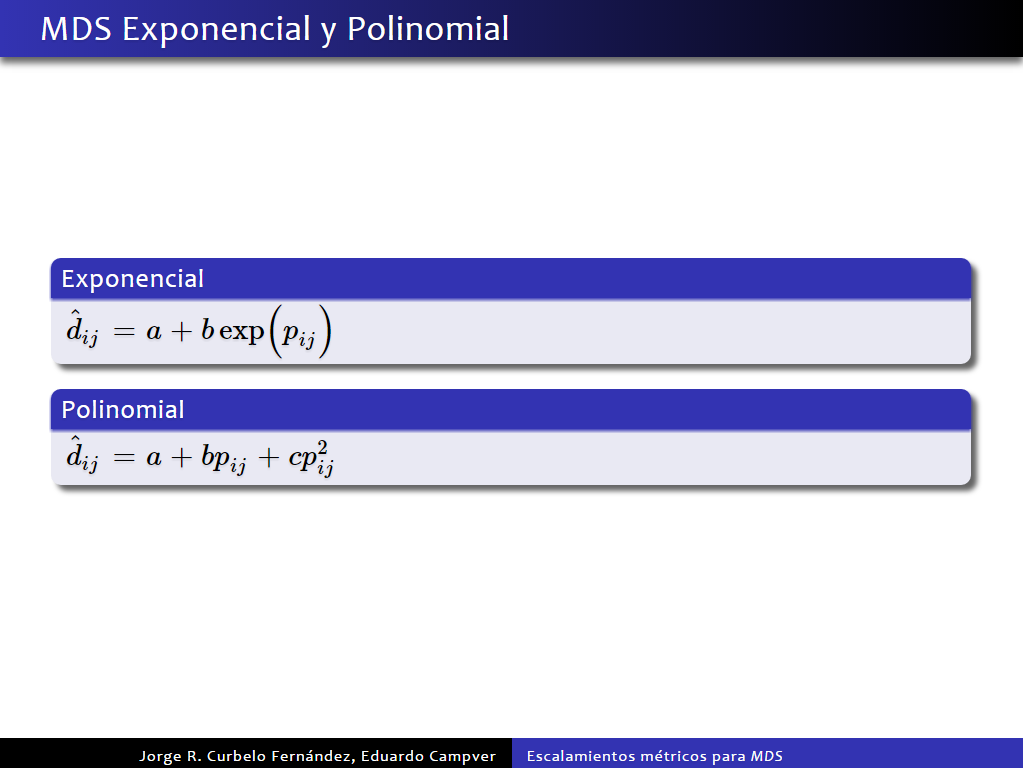
\includegraphics[width=\textwidth]{img/f1}
 				\caption{Primer frame}
 				\label{fig:frames_a}	
 			\end{subfigure}
 			\hspace*{\fill}
 			\begin{subfigure}[b]{0.3\textwidth}
 				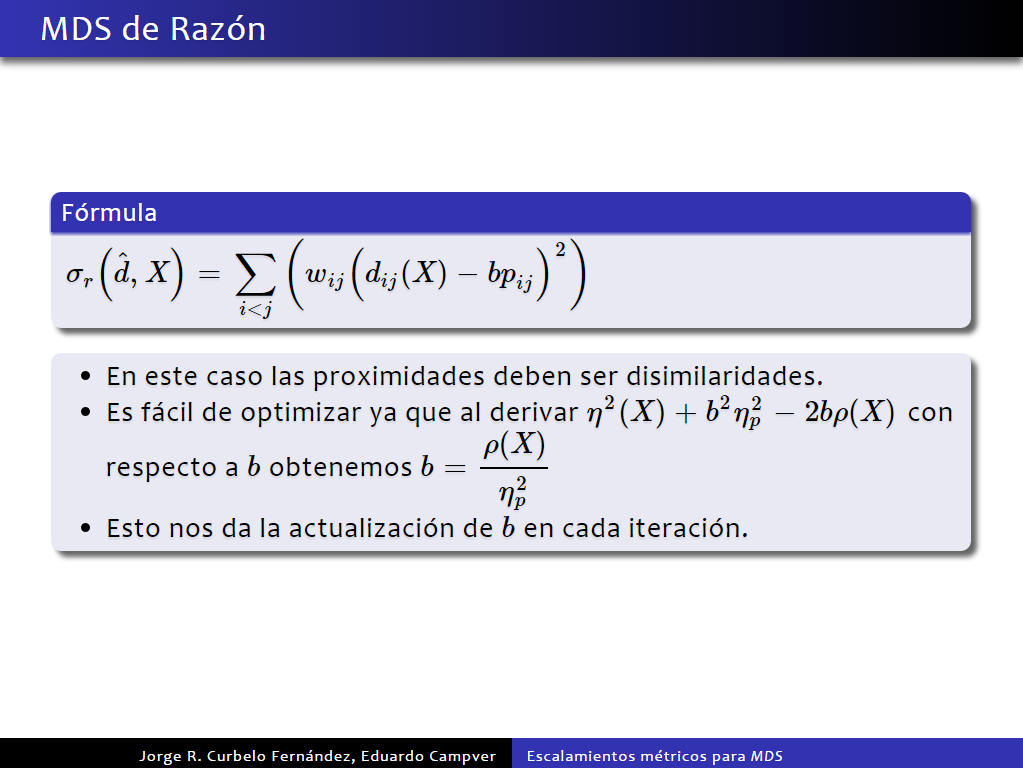
\includegraphics[width=\textwidth]{img/f2}
 				\caption{Segundo frame}
 				\label{fig:frames_b}	
 			\end{subfigure}
 			\hspace*{\fill}
 			\begin{subfigure}[b]{0.3\textwidth}
 				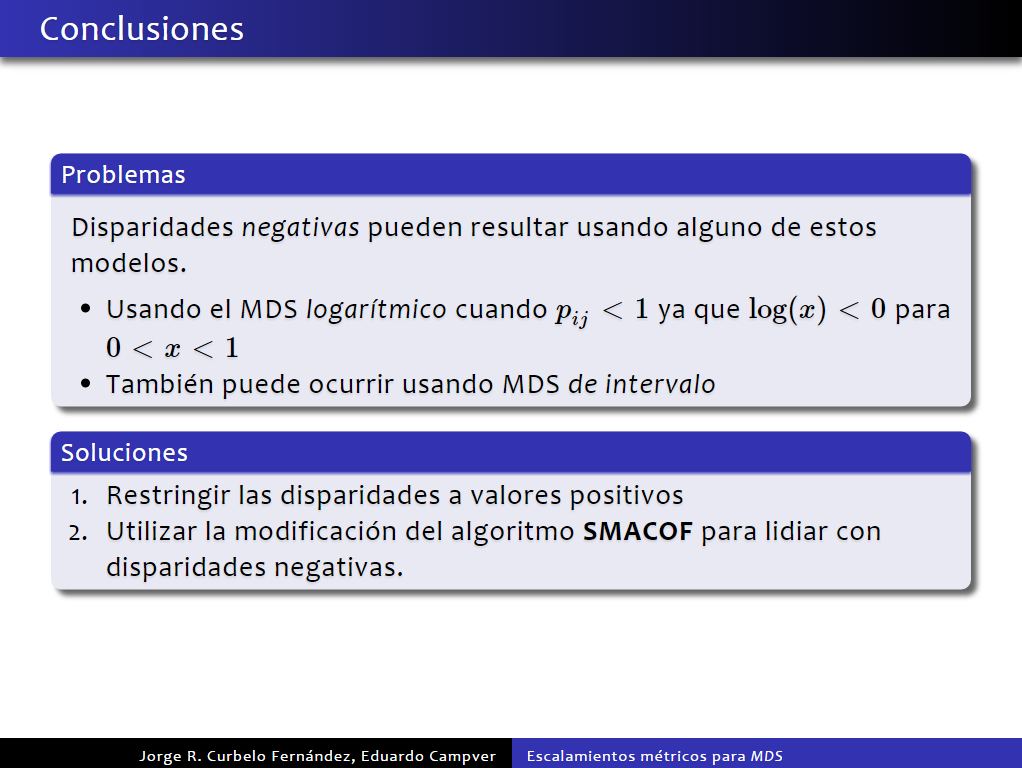
\includegraphics[width=\textwidth]{img/f3}
 				\caption{Tercer frame}
 				\label{fig:frames_c}	
 			\end{subfigure}			 			
 			\caption{Ejemplo de tres frames}
 			\label{fig:frames}
 		\end{figure}

 		\begin{definition}
 		\label{def:frame}
			Un \textbf{frame} es un conjunto de slides items y representa una diapositiva en la presentación. 
 		\end{definition}

 		Nótese que esta definición es distinta en \textit{Beamer}, donde un frame no es una diapositiva, sino un conjunto de ellas, que se muestran de forma tal que simulen una animación.

 		\begin{definition}
 		\label{def:slide_item}
 			Un \textbf{slide item}, es la base de los frames. Es un contenido que tiene definido un conjunto de overlays. 
 		\end{definition}

 		Por convenio, los slide items siempre están mostrados si no tienen un conjunto de overlays.

		Un ejemplo de slide item puede ser la imagen del frame en la fig \ref{fig:frame_video_image}, sin overlays.

		Las diapositivas y los contenidos de una presentación se exhiben con un orden. Por ejemplo, en la fig. \ref{fig:contents} se muestra un frame con tres contenidos que se ven en momentos distintos. A continuación se argumentarán las definiciones que se tuvieron en cuenta para especificar dicha ordenación.

 		\begin{figure}[tb]
 			\centering
 			\begin{subfigure}[b]{0.3\textwidth}
 				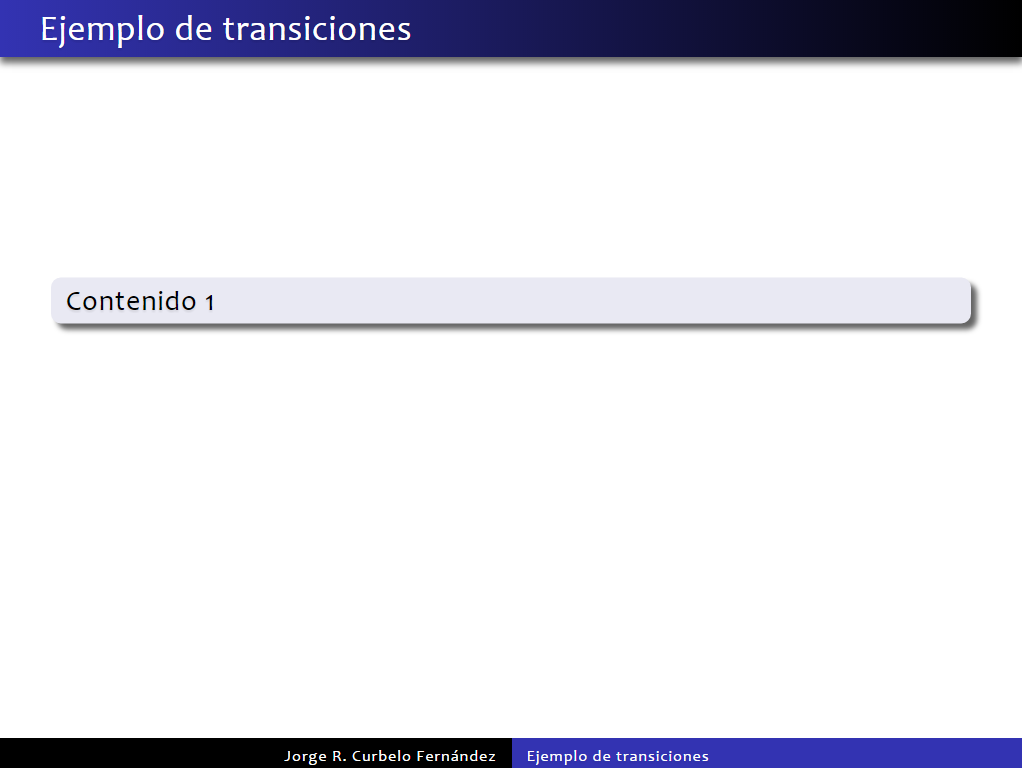
\includegraphics[width=\textwidth]{img/content1}
 				\caption{Slide 1}
 				\label{fig:contents_a}	
 			\end{subfigure}
 			\hspace*{\fill}
 			\begin{subfigure}[b]{0.3\textwidth}
 				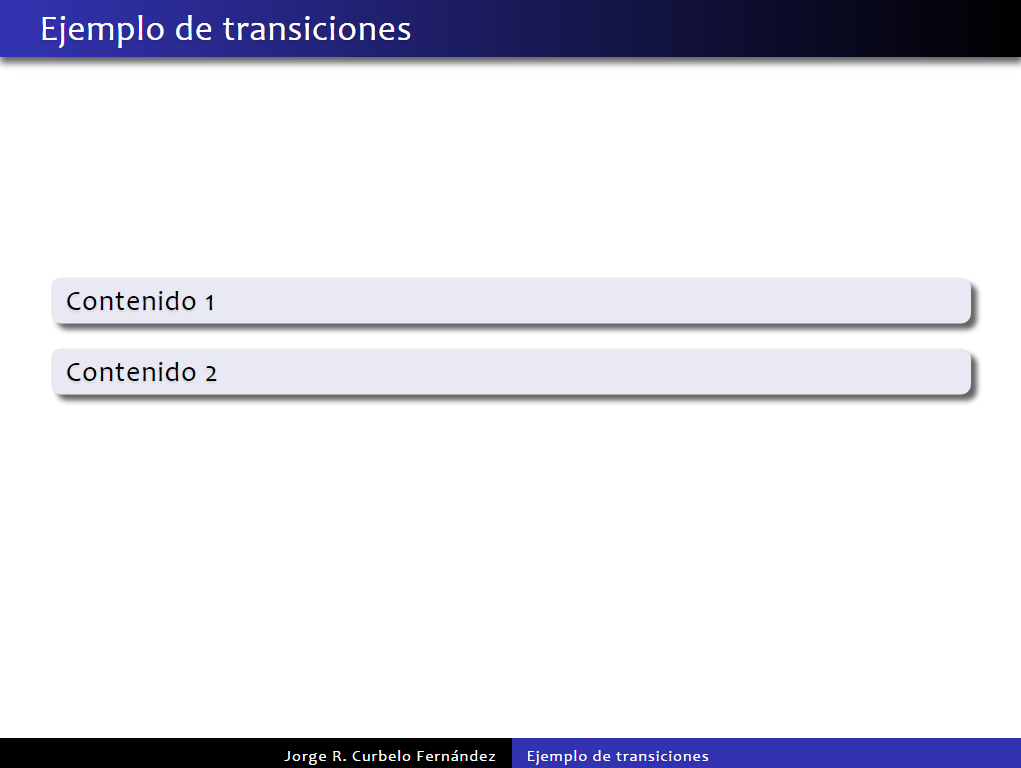
\includegraphics[width=\textwidth]{img/content2}
 				\caption{Slide 2}
 				\label{fig:contents_b}	
 			\end{subfigure}
 			\hspace*{\fill}
 			\begin{subfigure}[b]{0.3\textwidth}
 				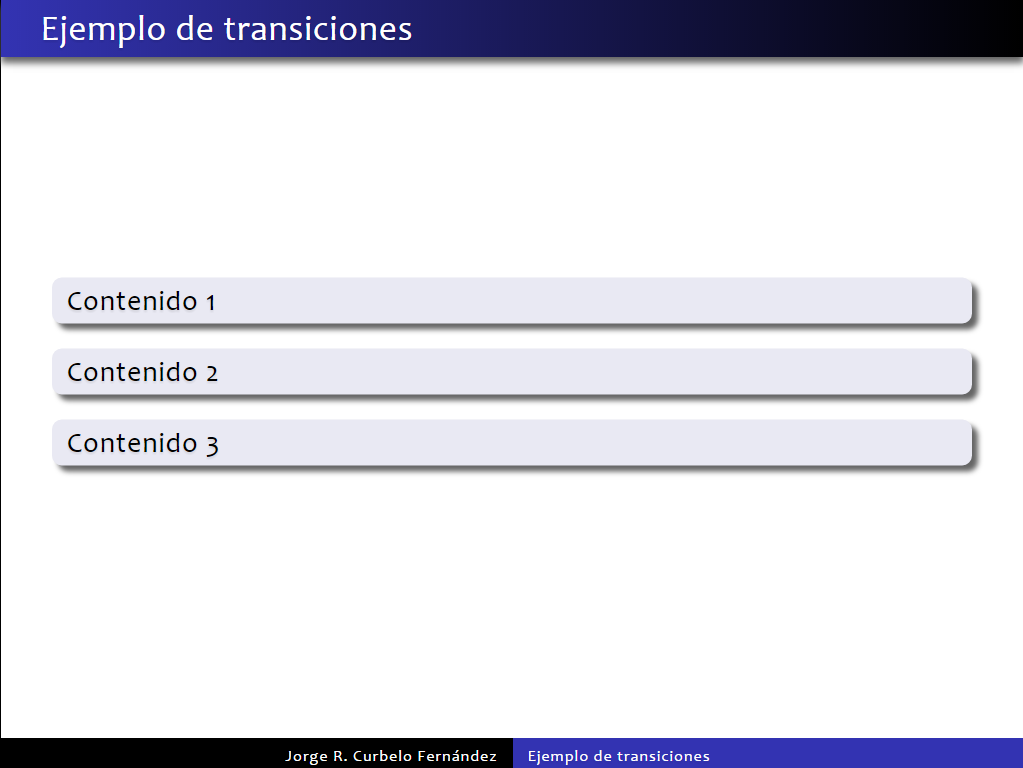
\includegraphics[width=\textwidth]{img/content3}
 				\caption{Slide 3}
 				\label{fig:contents_c}	
 			\end{subfigure}	 			
 			\caption{Ejemplo de un frame con tres contenidos mostrados en distintos slides}
 			\label{fig:contents} 
 		\end{figure}

 		\begin{definition}
 		\label{def:slide}
 			Un \textbf{slide} es un conjunto de slide items que se muestran simultáneamente en un frame.
 		\end{definition}
		
		Un frame puede tener varios slides y un slide se identifica con un número natural que simula el momento en que se mostrará su conjunto de slide items. Al estar los slides representados por enteros positivos, son ordenables. Decir que un slide es mayor que otro significa que ocurre después de otro. En \textit{Beamer} la definición de slide es distinta, ya que un slide representa una de las diapositivas de un frame.

		Por ejemplo, en la fig. \ref{fig:contents_b} el slide 2 es el conjunto formado por los dos primeros contenidos del frame, que son los mostrados. 

		Para determinar a qué slide pertenece un slide item se utilizan los overlays.				

 		\begin{definition}
 		\label{def:overlay}
 			Un \textbf{overlay} es un número natural ej: 3, o bien una secuencia de números naturales de la forma \texttt{inicio-final} ej: 3-5 que define el o los slides a los que pertenece un slide item.
 		\end{definition}

 		En caso de ser una secuencia de la forma \texttt{inicio-final} se toman las siguientes consideraciones: si no se especifica el slide \texttt{inicio} se asume 1 y si no se especifica el slide \texttt{final} se asume el último slide del frame. Muestras de estos casos se pueden ver en el ejemplo \ref{ex:overlay_set}. 		

 		\begin{definition}
 		\label{def:ovaerlay_set}
 			Un \textbf{conjunto de overlays} es una lista de ninguno o varios overlays separados por punto y coma (;).
 		\end{definition} 


		En el ejemplo \ref{ex:overlay_set} se expone la manera para definir un conjunto de overlays. Un slide item con los overlays de dicho ejemplo, indica que su contenido estará mostrado hasta el slide dos, no se mostrará en el tres, aparecerá en el cuatro, luego en el cinco se dejará de ver, reaparecerá desde el seis hasta el ocho, en el nueve se dejará de ver, y estará mostrado desde el diez hasta el final.  	

 		\begin{example}
 		\label{ex:overlay_set}
 			Un conjunto de overlays:
 			$$-2; 4; 6-8; 10-$$
 		\end{example}	

		% \begin{figure}[htb]%
		% 	\centering
		% 	$$-2; 4; 6-8; 10-$$
		% 	\caption{Ejemplo de un conjunto de overlays} 
		% 	\label{fig:overlay_set}
					
		% \end{figure} 		 						 		 				
		Los slide items definen un contenido en la presentación, a continuación se explica qué es un contenido y el comportamiento que puede tener.
		\begin{definition}
		\label{def:content}
			Un \textbf{contenido} es todo aquello que se muestre en las diapositivas, ya sea texto, imagen, audio, video o sus combinaciones posibles. 
		\end{definition}


		En la fig \ref{fig:frame_video_image} se expone un frame con varios contenidos: un video en la esquina superior izquierda, una imagen a su derecha y debajo tres bloques con texto.


 		\begin{figure}[tb]
 			\centering
 			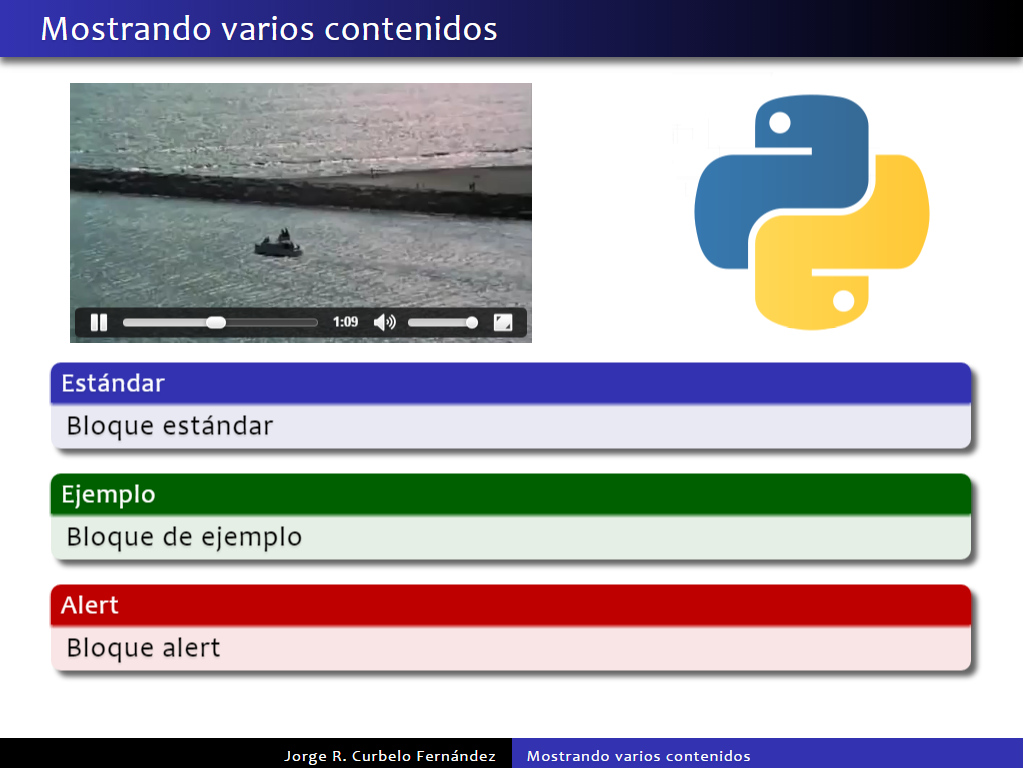
\includegraphics[width=12cm]{img/frame-video-image}
 			\caption{Ejemplo de un frame con contenidos}
 			\label{fig:frame_video_image}
 		\end{figure}

 		Un contenido puede estar oculto o mostrado, si se toman como ejemplo los tres contenidos del frame de la fig. \ref{fig:contents} se puede ver que en la fig. \ref{fig:contents_a} está mostrado el primer contenido y los otros dos están ocultos, mientras que en la fig. \ref{fig:contents_b} solo está oculto el tercero y en la fig. \ref{fig:contents_c} están motrados los tres contenidos.		

		\begin{definition}
		\label{def:show}
			\textbf{Mostrar un contenido} es la exhibición de imagen o de texto, la reproducción de audio o de video o cualquier combinación de estas posibilidades.
		\end{definition} 		


 		\begin{definition}
 		\label{def:transition}
 			Una \textbf{transición} es un cambio de slide o bien un cambio entre frames.
 		\end{definition}

 		\begin{definition}
 		\label{def:next_transition}
 			Una \textbf{transición siguiente} es el paso de un slide menor a uno mayor.
 		\end{definition} 		

 		\begin{definition}
 		\label{def:prev_transition}
 			Una \textbf{transición anterior} es el paso de un slide mayor a uno menor.
 		\end{definition}

 		Si se analiza una vez más la fig. \ref{fig:contents} se puede constatar que la fig. \ref{fig:contents_a}, la fig. \ref{fig:contents_b} y la fig. \ref{fig:contents_c} determinan tres slides distintos en dependencia de los instantes del frame. Un ejemplo de transición siguiente es el cambio de slides que provoca el paso del instante de la fig. \ref{fig:contents_a} a la fig. \ref{fig:contents_b}, mientras que una transición anterior es el efecto de cambiar el slide de la fig. \ref{fig:contents_c} al de la fig. \ref{fig:contents_b}.


		Para hacer uso de las transiciones con los overlays se introducen las siguientes definiciones.

		\begin{definition}
		\label{def:transition_func}
			Una \textbf{función de transición} en un slide item es una función que modifica el estado del contenido del slide item al ocurrir una transición.
		\end{definition}

		\begin{definition}
		\label{def:next_transition_func}
			Una \textbf{función de transición siguiente} en un slide item es una función que modifica el estado del contenido del slide item al ocurrir una transición siguiente.
		\end{definition}

		\begin{definition}
		\label{def:prev_transition_func}
			Una \textbf{función de transición anterior} en un slide item es una función que modifica el estado del contenido del slide item al ocurrir una transición anterior.
		\end{definition}

		Por defecto, se definen tres funciones de transición básicas: la función identidad, la función mostrar y la función ocultar.
		\begin{itemize}
		\label{it:basic_functions}
			\item \textbf{Función identidad}: No cambia el estado del contenido del slide item
			\item \textbf{Función mostrar}: Visualiza el contenido del slide item. Esta función no cumple totalmente con la definición \ref{def:show} de mostrar un contenido, ya que no es capaz de reproducir ni audios ni videos. La capacidad de hacer uso de elementos multimedias se argumenta en la sección \ref{subsec:sintaxis_extendida} 
			\item \textbf{Función ocultar}: Provoca que el contenido del slide item deje de ser visualizado
		\end{itemize}

		Como se vio en la definición \ref{def:slide_item}, un slide item está mostrado por defecto en todos los slides si no tiene un conjunto de overlays, pero de tenerlo se asume que está oculto en todos los slides, a no ser que sus overlays determinen otro comportamiento. En términos de las funciones elementales, esto se traduce en que todas las funciones de transición de un slide item (con overlays) por defecto son la función identidad excepto la primera, que es la función ocultar. 

		A continuación se define de una forma más detallada lo antes expuesto:

 		Sean \( I \), \( M \) y \( O \) la función identidad, la función mostrar y la función ocultar respectivamente


        Sea \( S_j \) un slide item, entonces la función de transición por defecto \( f_i \) de \( S_j \) para los slides \( 1 \dots n \) se define de la siguiente manera:


		\begin{equation}
		\label{eq:default}
			f_i = 
			\begin{cases}
				O, & \mbox{si }i = 1 \\
				I, & \mbox{si }1 < i \leq n.
			\end{cases}
		\end{equation}

		Seguidamente, se muestra otra definición de overlay usando las funciones elementales.

		\begin{definition}
		\label{def:new_overlay}

 			Un \textbf{overlay} es un número natural, o bien una secuencia de números naturales de la forma \texttt{inicio-final} que define una función de transición siguiente y una función de transición anterior.

		\end{definition}

		Usando esta definición, se puede ver el conjunto de overlays del ejemplo \ref{ex:overlay_set} de la manera siguiente:


		Sea \texttt{-2; 4; 6-8; 10-} dicho conjunto de overlays del slide item \( S_j \) que se encuentra en un frame con \( n \) slides. Entonces la función de transición \( f_i \) de \( S_j \) en el slide \( i \) es:

		\begin{equation}
		\label{eq:example}
			f_i = 
			\begin{cases}
				M, & \mbox{si }i = 1 \\
				I, & \mbox{si }i = 2  \\
				O, & \mbox{si }i = 3  \\
				M, & \mbox{si }i = 4  \\
				O, & \mbox{si }i = 5  \\
				M, & \mbox{si }i = 6  \\
				I, & \mbox{si } 6 < i \leq 8  \\
				O, & \mbox{si }i = 9  \\
				M, & \mbox{si }i = 10  \\
				I, & \mbox{si } 10 < i \leq n  \\
			\end{cases}
		\end{equation}

	% section definiciones (end)



	Luego de señalar las concepciones de \textit{Beampress}, se resalta su similitud con \textit{Beamer} en cuanto a \textit{Slides}, \textit{Overlays} y \textit{Frames}. Sin embargo, con la sintaxis para definir conjuntos de \textit{overlays} vista en el ejemplo \ref{ex:overlay_set} existe un problema: no es posible el uso de otras funciones de transición que no sean las elementales. Con estas funciones elementales no se puede incluir la reproducción de audios y videos ni el uso de animaciones, requisitos para \textit{Beampress} vistos en la sección \ref{sec:requerimientos_basicos_del_sistema_propuesto}. Por lo tanto conviene \textit{extender} o \textit{mejorar} la forma de definir los conjuntos de overlays.



	\subsection{Sintaxis extendida} % (fold)
	\label{subsec:sintaxis_extendida}
	

	Teniendo en cuenta los conceptos de slide item, overlay, conjunto de overlays y función de transición vistos en las definiciones \ref{def:frame}, \ref{def:overlay}, \ref{def:ovaerlay_set} y \ref{def:transition_func} respectivamente, se propone a continuación definir una extensión a la sintaxis vista en el ejemplo \ref{ex:overlay_set}. Como alternativa, se muestra en la fig. \ref{fig:json_format} una sintaxis para definir \textit{overlays} con cualquier \textit{función de transición}.

		\begin{figure}[htb]%
			\begin{lstlisting}%

{
    "número": {
        "siguiente": {
            "func": "nombre-de-función",
            "args": {...}
        },
        "anterior": {
            "func": "nombre-de-función",
            "args": {...}
        }
    }
}	
			\end{lstlisting}
		\caption{
			Formato JSON para un overlay con funciones de transición. 
			\label{fig:json_format} }
		\end{figure}


	Un overlay con esta sintaxis extendida es un JSON con las siguientes características:
	\begin{itemize}
		\item \texttt{número}: el número del slide
		\item \texttt{siguiente}: tiene como valores el nombre de la función de transición siguiente a utilizar, y sus argumentos
		\item \texttt{anterior}: tiene como valores el nombre de la función de transición anterior con sus argumentos
	\end{itemize}

	Una de las principales motivaciones para la creación de \textit{Beampress} fue el requerimiento de animaciones, audio y video detallado en la sección \ref{sec:requerimientos_basicos_del_sistema_propuesto}, para lo cual resulta imprescindible el manejo de dicha sintaxis transformada. Si se necesita reproducir un audio o un video se puede utilizar el ejemplo que se muestra en la fig. \ref{fig:ex_audio_video_syntax}. En dicho ejemplo se hará un \textit{fade in} para reproducir el video en el \textit{slide} 1 comenzando en el segundo 30. Lo mismo sucederá con el audio, pero en el \textit{slide} 2 y comenzando en el segundo 10.


	\begin{figure}[htb]%
		\begin{lstlisting}%

{
    "1": {
        "next": {
            "func": "fadeInVideo",
            "args": {
                "currentTime": "30"
            }
        },
        "prev": {
            "func": "fadeOutVideo",
            "args": {}
        }
    }
}

{
    "2": {
        "next": {
            "func": "fadeInAudio",
            "args": {
                "currentTime": "10"
            }
        },
        "prev": {
            "func": "fadeOutAudio",
            "args": {}
        }
    }
}
				
		\end{lstlisting}
		\caption{Ejemplo de uso de audio y video} 
			\label{fig:ex_audio_video_syntax}
		\end{figure}

		
		Como se vio en los overlays de la fig. \ref{fig:ex_audio_video_syntax}, las funciones de transición utilizadas (\texttt{fadeInVideo}, \texttt{fadeInAudio}) no son las funciones elementales. Esta sintaxis ampliada para definir overlays permite agregar nuevas funciones de transición además de las elementales, garantizando la extensibilidad de \textit{Beampress} que se verá con más detalles en el capítulo \ref{cha:extensibilidad}.


		Un ejemplo de un overlay con una función de transición distinta de las funciones elementales, se aprecia en la fig. \ref{fig:ball_code} y su ejemplo visual en la fig. \ref{fig:ball_visual}.



		\begin{figure}[htb]%
			\begin{lstlisting}%

{
    "3": {
        "next": {
            "func": "rollBallToLeft",
            "args": {}
        },
        "prev": {
            "func": "rollBallToRight",
            "args": {}
        }
    }
}
			\end{lstlisting}
		\caption{Ejemplo del empleo de una función de transición en un overlay} 
			\label{fig:ball_code} 
		\end{figure}	




 		\begin{figure}[tb]
 			\centering
 			\begin{subfigure}[b]{0.3\textwidth}
 				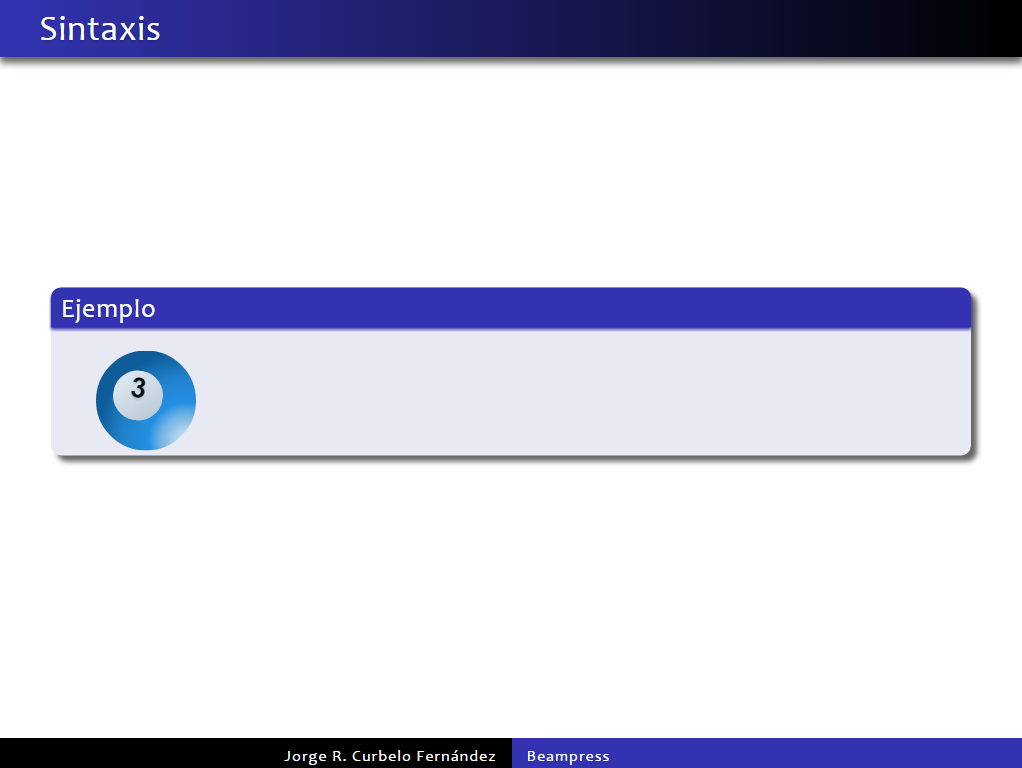
\includegraphics[width=\textwidth]{img/ball-left}
 				\caption{En la izquierda}
 				\label{fig:ball_visual_a}	
 			\end{subfigure}
 			\hspace*{\fill}
 			\begin{subfigure}[b]{0.3\textwidth}
 				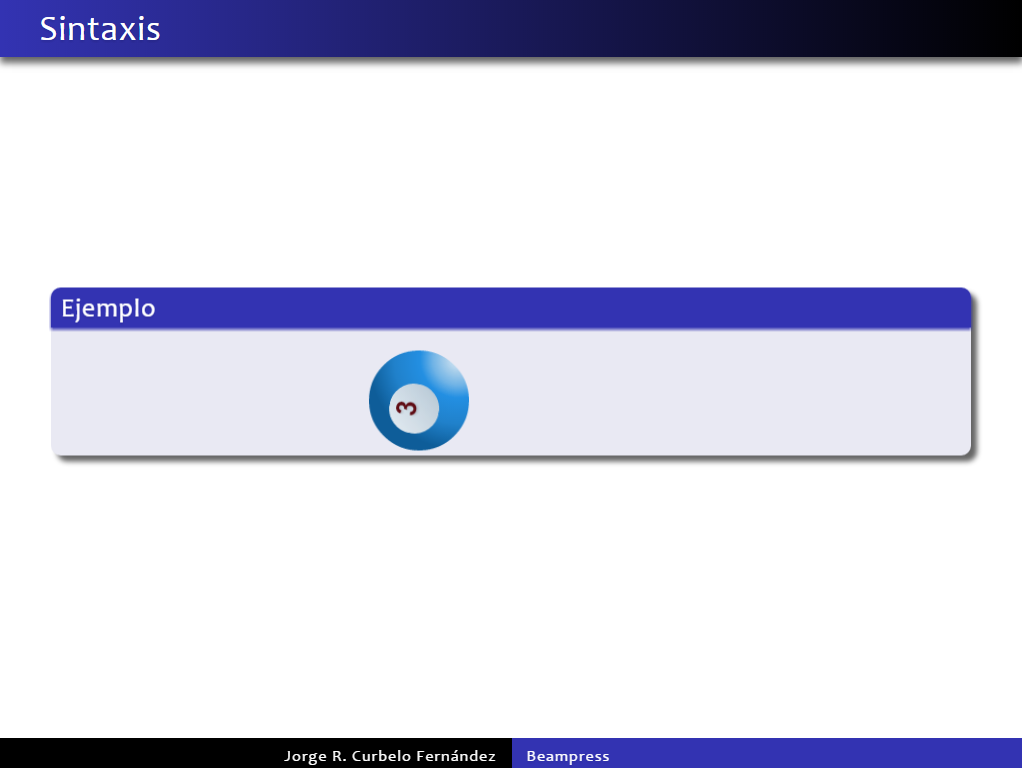
\includegraphics[width=\textwidth]{img/ball-middle}
 				\caption{En el medio}
 				\label{fig:ball_visual_b}	
 			\end{subfigure}
 			\hspace*{\fill}
 			\begin{subfigure}[b]{0.3\textwidth}
 				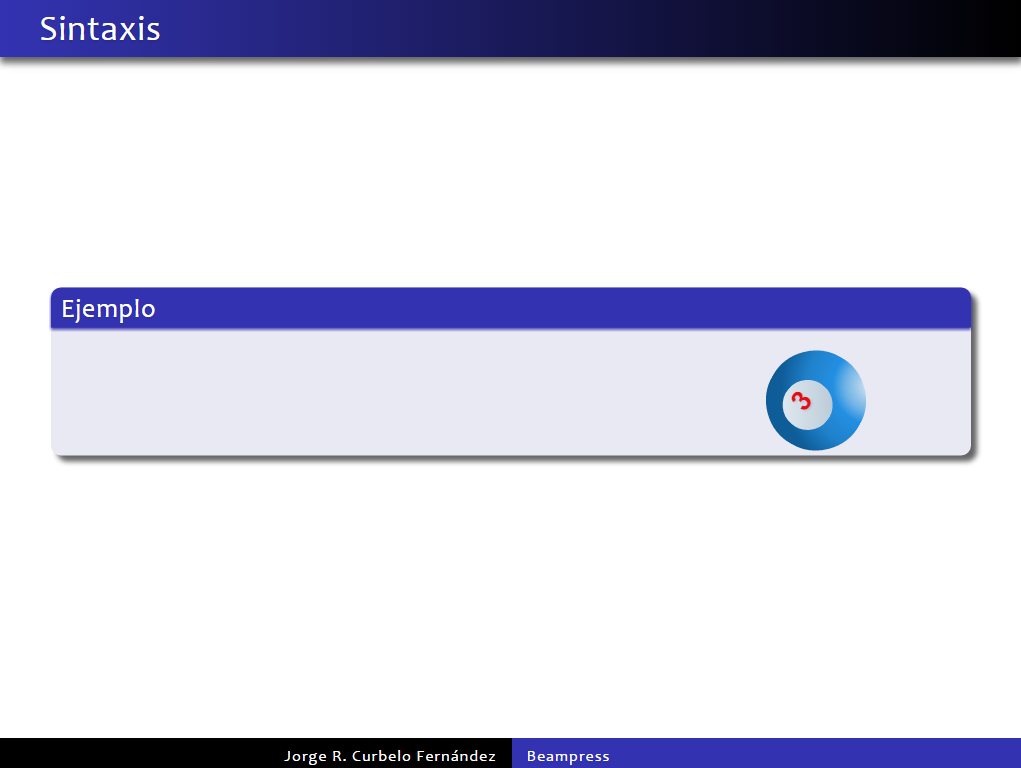
\includegraphics[width=\textwidth]{img/ball-right}
 				\caption{En la derecha}
 				\label{fig:ball_visual_c}	
 			\end{subfigure}	  			
 			\caption{Ejemplo visual de la animación definida con el overlay de la fig. \ref{fig:ball_code}}
 			\label{fig:ball_visual} 
 		\end{figure}	


	Con el empleo de esta sintaxis, es posible definir las funciones de transición de los \textit{Frames}. En la fig. \ref{fig:frame_trans} se muestra un ejemplo de esto.

		\begin{figure}[htb]%
			\begin{lstlisting}%

{
    "func": "slowShowFrame",
    "args": {}
}

{
    "func": "slowHideFrame",
    "args": {}
}
			\end{lstlisting}
		\caption{
			Funciones de transición para un frame. 
			\label{fig:frame_trans} }
		\end{figure}	

	

		Con la implementación de las ideas anteriormente explicadas, se resuelve la mayoría de las dificultades analizadas en la sección \ref{sec:proyecto_delta}, referentes al Proyecto Delta, o sea, la inclusión de videos, audios y animaciones en la proyección de diapositivas. Sin embargo, permanece el obstáculo de la distancia entre el presentador y la computadora que contiene la presentación. En la próxima sección, se presenta el servidor web \textit{Beampressk}, que soluciona dicha dificultad.
	% section sintaxis_extendida (end)

	\section{Definiciones de Beampressk} % (fold)
	\label{sec:definiciones_de_beampressk}

		 En esta sección se exponen las definiciones que dan solución a la dificultad del Proyecto Delta en cuanto a la distancia entre el presentador y la computadora que contiene la presentación. Estas son: vista de presentación, control y modificación dinámica de la presentación, posibilidad de mostrar mensajes de texto, live feed y vista de control, todo lo cual se argumenta en las definiciones \ref{def:presentation_view}, \ref{def:dynamic_control}, \ref{def:presentation_modification}, \ref{def:message}, \ref{def:live_feed} y \ref{def:control_view} respectivamente. %También se argumentarán los recursos vistos en la sección \ref{sec:beampressk} que determina \textit{Beampressk} al ser concebido como \textit{API REST}.

		\begin{definition}
		\label{def:presentation_view}
			La \textbf{vista de presentación} muestra la presentación. 
		\end{definition}

		La vista de presentación puede ser visualizada o accedida desde diferentes dispositivos. Esto permite que una misma presentación se muestre simultáneamente en distintos lugares.

		Como se vio en las definiciones \ref{def:next_transition} y \ref{def:prev_transition} una presentación cuenta con transiciones siguiente y anterior, estas a su vez realizan un cambio de slide o un cambio de frame. \textit{Beampressk} brinda la posibilidad de efectuar dichas transiciones desde el dispositivo que contiene la presentación o desde cualquier otro.


		\begin{definition}
		\label{def:dynamic_control}
			\textbf{Controlar de forma dinámica una presentación} es la posibilidad de realizar transiciones por el presentador en el momento que él determine.
		\end{definition}


		% A continuación se definen elementos que son derivados de estas dos primeras definiciones.

		Como se vio en la sección \ref{sec:requerimientos_basicos_del_sistema_propuesto}, uno de los requisitos para la propuesta de este trabajo es que la presentación esté en ámbito web para lograr una interacción con otros \textit{servicios web} y en el caso particular de las presentaciones del Proyecto Delta se trata de mostrar en el medio de la presentación los mensajes de texto que envía el público. Para esto se define lo siguiente: 

		\begin{definition}
		\label{def:presentation_modification}
			\textbf{Modificar la presentación} es la capacidad de variar, agregar o eliminar un contenido mientras transcurre la presentación.
		\end{definition}

		Cuando se habla de \textit{variar} puede ser modificar el volumen de un contenido multimedia, la posición de una imagen o el tamaño de un texto, entre otros parámetros.

		% A continuación se definen elementos derivados de la definición.

		\begin{definition}
		\label{def:message}
			\textbf{Mostrar un mensaje en la presentación} es añadir un contenido de forma dinámica con el texto de dicho mensaje en el frame que se está mostrando. 
		\end{definition}

		La acción de enviar este texto es independiente de la presentación, y el presentador decide el momento en que será exhibido y ocultado. En la fig. \ref{fig:msg} se visualiza un mensaje de texto en un frame.


		\begin{figure}[tb]
			\centering
			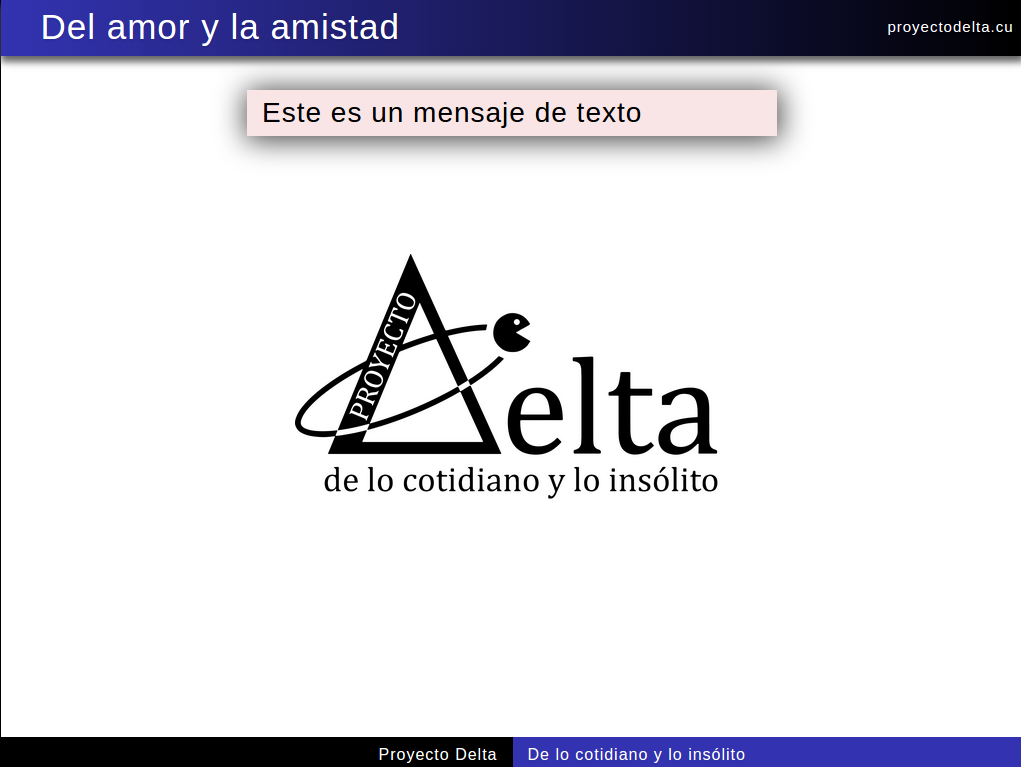
\includegraphics[width=12cm]{img/text_msg}
			\caption{Ejemplo de un mensaje de texto mostrado en la presentación}
			\label{fig:msg}
		\end{figure}

		Otra necesidad que se constata en la sección \ref{sec:proyecto_delta} es la capacidad de incorporar en la presentación un \textit{live feed}.

		\begin{definition}
		\label{def:live_feed}
			Un \textbf{live feed} es la inserción en la presentación de un contenido que consiste en la imagen que filma una cámara y el audio que registra un micrófono.
		\end{definition}

		En la fig. \ref{fig:live_feed} se muestra un ejemplo de live feed.

		\begin{figure}[tb]
			\centering
			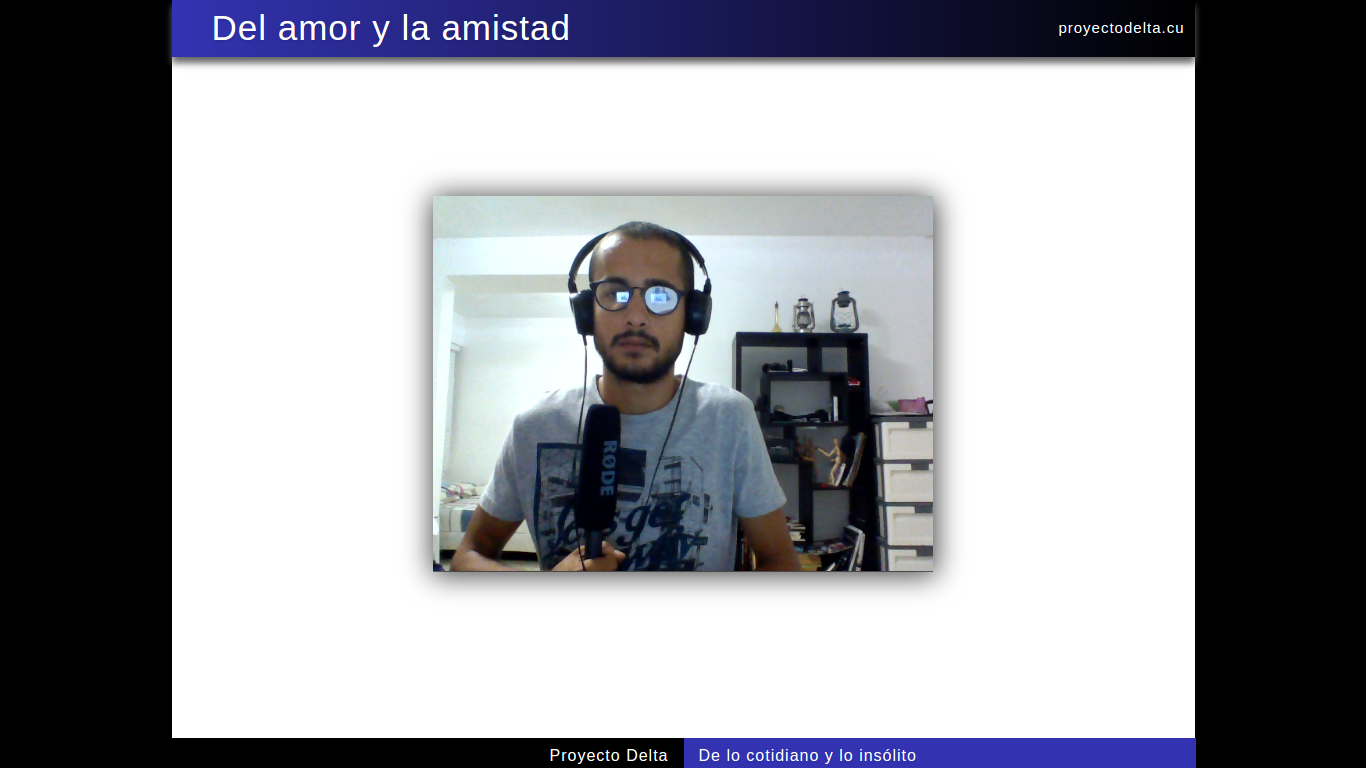
\includegraphics[width=12cm]{img/live_feed}
			\caption{Ejemplo de live feed}
			\label{fig:live_feed}
		\end{figure}

		Finalmente, se define el componente que controla la presentación teniendo en cuenta las definiciones \ref{def:dynamic_control}, \ref{def:presentation_modification}, \ref{def:message} y \ref{def:live_feed}.

		\begin{definition}
		\label{def:control_view}
			La \textbf{vista de control} manipula de forma dinámica una presentación y la modifica, siendo capaz de reorganizarla, de agregar contenidos como mensajes de texto y un live feed, de modificar algunas propiedades como el volumen de un video, y de eliminar un contenido como un mensaje de texto previamente agregado en la presentación. 
		\end{definition}		
		
		La vista de control es independiente de la vista de presentación. Se puede mostrar en el dispositivo que contiene la presentación o en cualquier otro, dando la opción de ser visualizada al mismo tiempo en varios lugares. Esto significa que pueden existir varios \textit{controladores} manipulando una misma presentación.

		Un requisito de vital importancia es que exista un canal de comunicación bidireccional entre la vista de presentación y la vista de control, para que las acciones y las respuestas entre las dos vistas tengan efecto instantáneo. Para esto se definen los mensajes de \textit{acción} y \textit{respuesta} en la tabla \ref{tab:messages}.

			\begin{table}[b]
				\caption{Mensajes de comunicación entre la vista de control y la vista de presentación}
				\label{tab:messages}
				\centering
			
				\begin{tabular}{| m{2cm} | m{3cm} | m{2.5cm} | m{3cm} |}
				\hline
			
				\hline
					\textbf{Vista Control} & \textbf{Acción} & \textbf{Vista \newline Presentación} & \textbf{Acción} \\
				\hline
					\texttt{siguiente} & Realiza una transición siguiente & \texttt{respuesta actualiza} & Actualiza la información en la vista de control. La información está integrada por el frame y el slide actual, así como por el nivel del volumen, y si está o no mostrado el live feed o algún mensaje de texto  \\ \cline{1-2}
				% \hline
				% \hline
					\texttt{anterior} & Realiza una transición anterior &   &  \\ \cline{1-2}
				% \hline

				% \hline
					\texttt{volumen} & Ajusta el volumen con el valor especificado en el contenido del mensaje &  &  \\ \cline{1-2}
				% \hline	

				% \hline
					\texttt{live feed} & Muestra / oculta un live feed &  &  \\ \cline{1-2}
				% \hline

				% \hline
					\texttt{message} & Muestra / oculta un mensaje &  &  \\ \cline{1-2}
				% \hline

				% \hline
					\texttt{go to} & Se muestra el frame y el slide que se especifica en el contenido del mensaje &  &  \\ 
				\hline																																
			
				\hline
				\end{tabular}
			\end{table}	


		En este capítulo se analizaron, de \textit{Beampress}, los conceptos de presentación, slide, slide item, overlay y contenido, así como las transiciones anterior y siguiente y la necesidad de una sintaxis extendida para definir cualquier función de transición. También se detallaron otras definiciones que pertenecen a \textit{Beampressk}, como vistas de presentación y de control, la capacidad de modificar y controlar la presentación, y la instantaneidad que se logra en la comunicación entre las dos vistas.

		Seguidamente se detallan las implementaciones de \textit{Beampress}: un plugin de JQuery, y de \textit{Beampressk}: un servidor web implementado en Flask.


	

% chapter fundamentos_conceptuales (end)




